% !TEX program = lualatex
\documentclass[../../main.tex]{subfiles}
\begin{document}

\subsection{Provisioning a new device}%
\label{sub:provisioning_a_new_device}
Assuming rpi3b+ as to always just run PXE boot. Though if using an older rpi unit use 
\mintinline{bash}{bootbin.sh} to setup an sdcard up with the bootcode.bin file which
enables older rpis to PXE boot.

PXE boot server is hosted on an rpi. A new device will boot a default raspbian buster image
which mounts an nfs share from the development host which have the current sdcard image that 
should be deployed. On the same share there is a script, \mintinline{bash}{boot.sh}, which is
run using a cron job during startup.\\

\todo{figur} 
\usegdlibrary {force}
\begin{figure}[h]
\begin{center}
\begin{tikzpicture}[]
	\graph [spring layout,component sep=2cm] {
		"switch" -- {
			"PXEBOOT server",
			"build host",
			"New device
		}
	};
\end{tikzpicture}
\end{center}
\caption{}%
\label{fig:}
\end{figure}



When a device boots the mender image for the first time it will show up as pending on the mender
host interface as can be seen in figure \ref{fig:mender-ui-pending}.
Here it can be accepted as a authorized device.
This is under the assumption that local network on which the developer host attached is secure.

\begin{figure}[h]
	\centering
	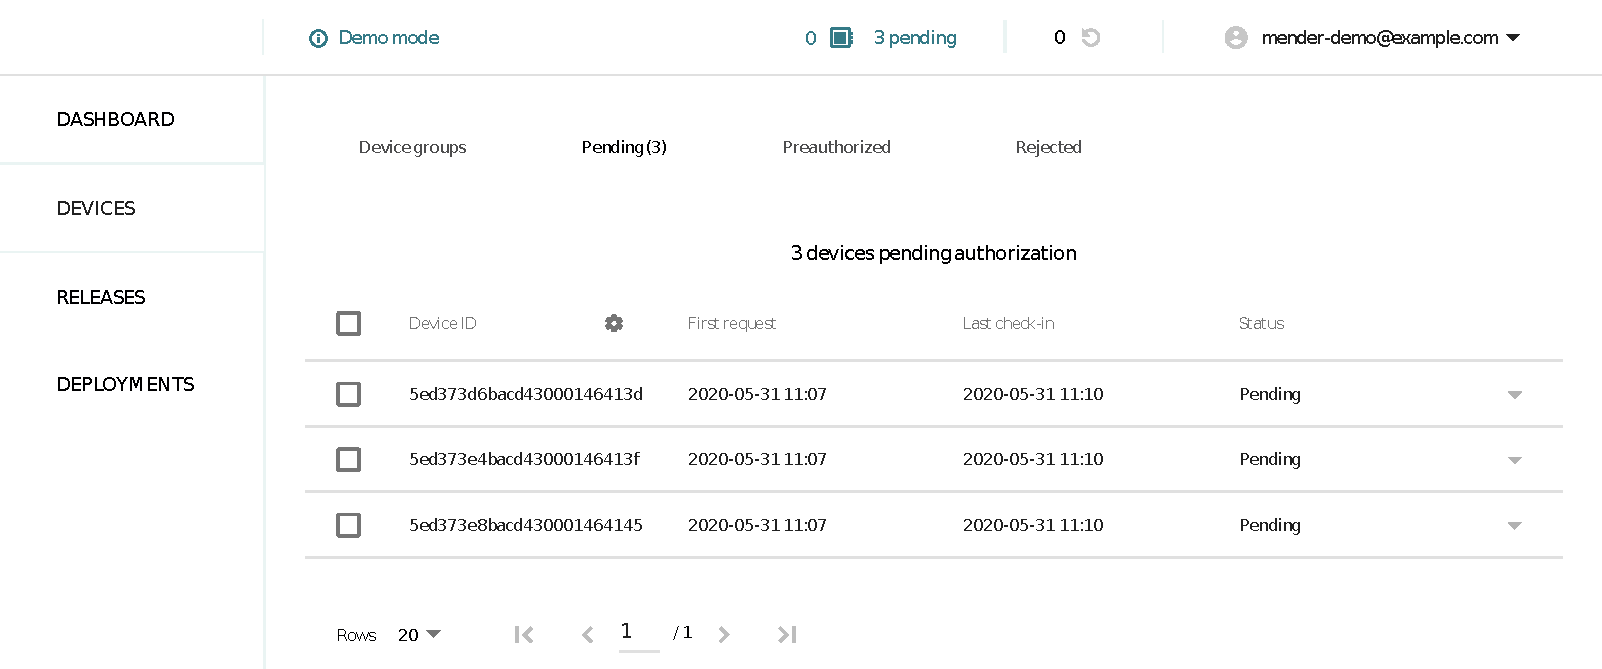
\includegraphics[width=1\linewidth]{img/mender-ui-pending-edited.pdf}
	\caption{Mender interface when device is pending}%
	\label{fig:mender-ui-pending}
\end{figure}

\subsection{Updating existing device}%
\label{sub:updating_existing_device}

Updating a device is taken of by the mender server. When compiling a sdcard image using yocto,
a mender artefact is also generated, this can be uploaded to the mender server.
The artefact can then be assigned devices or groups, where any device in an assigned group will
receive the update the next time the deployed device polls the mender server.

\todo{More about how mender does this and what to do when an update false}


\subsection{Tasks}%
\label{sub:tasks}

Tasks are deployed using the mender update module and deploying a task have been made idempotent
to not insure that a device will not try to execute the same task twice over.

A mender update module is an executable located in \texttt{/usr/share/mender/modules/v3}
which takes 2 arguments, state and files.

For this project we assume that any needed program is existing on the deployed device,
so a update module is made that adds tasks as cron jobs.

Tasks are visible in the mender inventory.

\subsection{Docker}%
\label{sub:docker}

Instead of porting projects mender already has a docker update module. This of course reduce
the requirement for porting project at the expense of greater overhead, connected with running
containers.

The custom kernel module is still needed on the deployed device, but other than that it only needs
the docker service.

A mclurs docker file can be seen in listing \ref{lst:mclurs-docker}.

\begin{listing}[h]
\inputminted{docker}{/home/aske/Bachelor/DockerMCLURS/Dockerfile}
\caption{A docker file that enables the MCLURS project to run in a dockerdocker  container.}
\label{lst:mclurs-docker}
\end{listing}

The docker container can then be build and pushed to dockerhub.
A mender artifact can then be generated as shown in listing \ref{lst:docker-mender-push}.
The artefact can be uploaded the mender server and from there a deployment can be created
to any device matching \mintinline{bash}|${DEVICE_TYPE}|.

\begin{listing}[h]
\begin{minted}{bash}
docker build . -t mclurs
docker push ${ID}/${REPO}:mclurs
docker-artifact-gen -n ${ARTIFACT_NAME} -t ${DEVICE_TYPE} -o ${OUTPUT_PATH} ${DOCKER_IMAGES}
\end{minted}
\caption{Generate mender artefact for the docker mender update module.}
\label{lst:docker-mender-push}
\end{listing}





Demo docker with c-sense-hat interacting with hardware.

\end{document}
